%% beamer-mpg
%% A beamer example LaTeX file partially adapted to the MPG Corporate Design
%% 
%%     For internal use at MAX-PLANCK-GESELLSCHAFT e.V. only!
%% 
%%     WITHOUT ANY WARRANTY; without even the implied warranty of
%%     MERCHANTABILITY or FITNESS FOR A PARTICULAR PURPOSE.
%% 
%% 
%% MPG Corporate Design Manual 2008 (3rd edition)
%% See Max Planck Intranet: https://intranet.mpg.de/gv/abt06/Referat_Vb/Documents/CD%20Manual%202008.pdf
%% 
%%
%% beamer im Seminarraum: 1024/768 Benq MP622
%% 
%\documentclass[german,handout]{beamer}
\documentclass[german]{beamer}
\usepackage[english,ngerman]{babel}
\usepackage[T1]{fontenc}
\usepackage[latin9]{inputenc}
\usepackage{color}
\setcounter{secnumdepth}{3}
\setcounter{tocdepth}{3}
\usepackage{graphicx}
\usepackage{booktabs}
\usepackage{multirow}
\usepackage{rotating}
\usepackage{listings}
\usepackage{pythonhighlight}
\usepackage[pdf]{pstricks}
\usepackage{tikz}
%% for the blitz symbol
\usepackage{ulsy}
\newcommand{\ra}{\text{$\rightarrow$}}
 \newcommand{\Pause}{}
% \newcommand{\Pause}{\pause}
\DeclareMathOperator*{\argmin}{arg\,min}
\DeclareMathOperator*{\argmax}{arg\,max}

\usepackage{pgfpages}

% for [handout]
%\setbeameroption{show notes} 
%\pgfpagesuselayout{4 on 1}[a4paper,border shrink=5mm]

%% fix acroread/tikz bug, see http://tex.stackexchange.com/questions/9261/using-opacity-in-tikz-causes-strange-rendering-in-acrobat
\pdfpageattr{/Group <</S /Transparency /I true /CS /DeviceRGB>>} 

\newcommand{\placeholder}{\rule{0pt}{1pt}}
\newlength{\stimsize}
\newlength{\peopleheight}

%% uncomment this to show notes on second screen




%% see http://www.tug.org/pracjourn/2010-1/dohmen/dohmen.pdf for dual-screen presentations including slides + notes on the presenter's screen (=second screen)!
%% e.g. for a 1366x768 laptop screen resolution and a 1024x768 VGA Beamer resolution the xrandr command is
%% xrandr --output VGA1 --mode 1024x768 --scale 0.6670x0.6670 --pos 0x128
%% see the PDF for how to calculate the scale and pos arguments!
%%
%% screen resolutions at MPIDS Bernsteinzimmer: 2x Full HD 1920x1080 (?)!!


%% MPG green (Pantone 328), see CD manual 2008, p. 12
\definecolor{mpg-green}{cmyk}{1,0,0.57,0.3}

%% MPG grey (Pantone 427), see CD manual 2008, p. 12
\definecolor{mpg-grey}{cmyk}{0,0,0.6,0.15}

\usetheme{Madrid}

%% remove slide numbers (must be AFTER theme init)
\setbeamertemplate{footline}
{
  \leavevmode%
  \hbox{%
  \begin{beamercolorbox}[wd=.333333\paperwidth,ht=2.25ex,dp=1ex,center]{author in head/foot}%
    \usebeamerfont{author in head/foot}\insertshortauthor
  \end{beamercolorbox}%
  \begin{beamercolorbox}[wd=.333333\paperwidth,ht=2.25ex,dp=1ex,center]{title in head/foot}%
    \usebeamerfont{title in head/foot}\insertshorttitle
  \end{beamercolorbox}%
  \begin{beamercolorbox}[wd=.333333\paperwidth,ht=2.25ex,dp=1ex,right]{date in head/foot}%
    \usebeamerfont{date in head/foot}\insertshortdate{}\hspace*{2em}
%    \insertframenumber{} / \inserttotalframenumber\hspace*{2ex} 
  \end{beamercolorbox}}%
  \vskip0pt%
}

%% Beamer color theme
\usecolortheme[cmyk={1,0,0.57,0.3}]{structure} 

%% Use Venturis ADF instead of Bodoni
\setbeamerfont{structure}{family*=yvt}


%% use MPG green also for alerted text
\setbeamercolor{alerted text}{fg=mpg-green}

\beamertemplatenavigationsymbolsempty
%% custom Section page : no 'Section X' text
\setbeamertemplate{section page}
{
  \begin{centering}
    \begin{beamercolorbox}[sep=12pt,center]{part title}
      \usebeamerfont{section title}\insertsection\par
    \end{beamercolorbox}
  \end{centering}
}

%% custom Subsection page: no 'Subsection X.Y' text
\setbeamertemplate{subsection page}
{
  \begin{centering}
    \begin{beamercolorbox}[sep=8pt,center]{part title}
      \usebeamerfont{subsection title}\insertsubsection\par
    \end{beamercolorbox}
  \end{centering}
}

%% shows the section page at the begin of each section ...
\AtBeginSection[]
{
  \frame{\sectionpage}
}

%% shows the subsection page at the begin of each subsection ...
\AtBeginSubsection[]
{
  \frame{\subsectionpage}
}


%% Activate this for production
%% open pdf in fullscreen mode (if in beamer mode, default)
%\mode<beamer>{  \hypersetup{pdfpagemode=FullScreen} }


\begin{document}
\lstset{language=Python,
  showstringspaces=false,
  frame=shadowbox,
  style=mypython,
  basicstyle=\ttfamily\footnotesize
}
%  numbers=left}
%  numberstyle=\tiny,
 
\institute[MPI DS]{
  Max-Planck-Institute for Dynamics and Self-Organization
}
\title[C and Python]{Interfacing C code from Python}
\author{Matthias~Ihrke}

\date{26.4.2012}
\titlegraphic{
\includegraphics[height=2cm]{pics/cython2}}


\begin{frame}[label=mytitle]
  \titlepage 
\end{frame}

%------------------------------------------------------------------------------
%----------------------------------------------------------------------
%SLIDE -

\begin{frame}[fragile]{C and Python}

\begin{block}{What?}
  Call compiled code written in C from within Python (works also for
  C++ but I will focus on C).
\end{block}

\begin{block}{Why?}
\begin{itemize}
\item Python is elegant, C can be ugly 
\item Python is slow, compiled code is fast
\end{itemize}

Conclusion:
\begin{itemize}
\item use high-level, easy-to-read code for the framework (e.g.,
  parameter scans, plotting, data-analysis)
\item use a C-module for the calculation-intense parts of the program
\end{itemize}

\end{block}
\end{frame}

%----------------------------------------------------------------------
%SLIDE -

\begin{frame}[fragile]{Example 1: File I/O}
  To illustrate this point, we implement reading a sequence of numbers
  from a comma-separated file ({\tt .csv}) of the format
  \begin{semiverbatim}
    12.4,43.43215432,321.455,12.3245432 ...
  \end{semiverbatim}
\end{frame}
%----------------------------------------------------------------------
%SLIDE -
\begin{frame}[fragile]{Example 1}
  \framesubtitle{Read a file of comma-separated values}

  Solution in C:
  \lstinputlisting[language=C,basicstyle=\tiny,caption=csv.c]{../examples/csv/csv.c}

\end{frame}

%----------------------------------------------------------------------
%SLIDE -
\begin{frame}[fragile]{Example 1}
  \framesubtitle{Read a file of comma-separated values}

  Solution in Python:
  \lstinputlisting[language=Python,caption=csv.py]{../examples/csv/csv.py}

  or with numpy
  \lstinputlisting[language=Python,caption=csv\_numpy.py]{../examples/csv/csv2.py}

\ra Roughly one order of magnitude reduction in code-length

\ra enormous speedup in writing (and debugging!) the code 
\end{frame}
%----------------------------------------------------------------------
%SLIDE -

\begin{frame}{Example 2: Primality test}
  \framesubtitle{Is 715827883 a prime number? (yes, Wagstaff prime)}
  
  To determine whether an integer $n$ is a prime number, we implement
  a very basic algorithm:
  \begin{block}{Algorithm 1: Basic Primality test}
    Loop through all numbers $1<i<n$ and return ``false'' if 
    for any $i: n\text{ mod }i=0$. Otherwise, return ``true''.
  \end{block}
  
  \begin{block}{Properties of this example}
    \begin{itemize}
    \item computationally intense, but requires only a single number
      as input and output
    \item cannot really be done in numpy (memory problems, at least
      $\approx 6$ GB)
    \end{itemize}
  \end{block}

\end{frame}
\begin{frame}[fragile]{Example 2: Primality test}
  \framesubtitle{Is 715827883 a prime number?}

  Solution in Python:
  \lstinputlisting[language=Python,caption=prime.py]{../examples/prime/prime.py}
\end{frame}

%----------------------------------------------------------------------
%SLIDE -

\begin{frame}[fragile]{Example 2: Primality test}
  \framesubtitle{Is 715827883 a prime number?}

  Solution in C:
  \lstinputlisting[language=C,caption=prime.c]{../examples/prime/prime.c}

\end{frame}
%----------------------------------------------------------------------
%SLIDE -
\begin{frame}[fragile]{Example 2: Primality test}
  \framesubtitle{Runtime Comparison}

\begin{minipage}{.45\textwidth}
\begin{block}{C}
7.439 sec
\end{block}
\end{minipage}
\hfill
\begin{minipage}{.45\textwidth}
\begin{block}{Python}
58.225 sec
\end{block}
\end{minipage}

Roughly one order of magnitude speedup.
\end{frame}



%----------------------------------------------------------------------
%SLIDE -
\begin{frame}[fragile]{The best of both worlds}
Allow Python to access your C-code

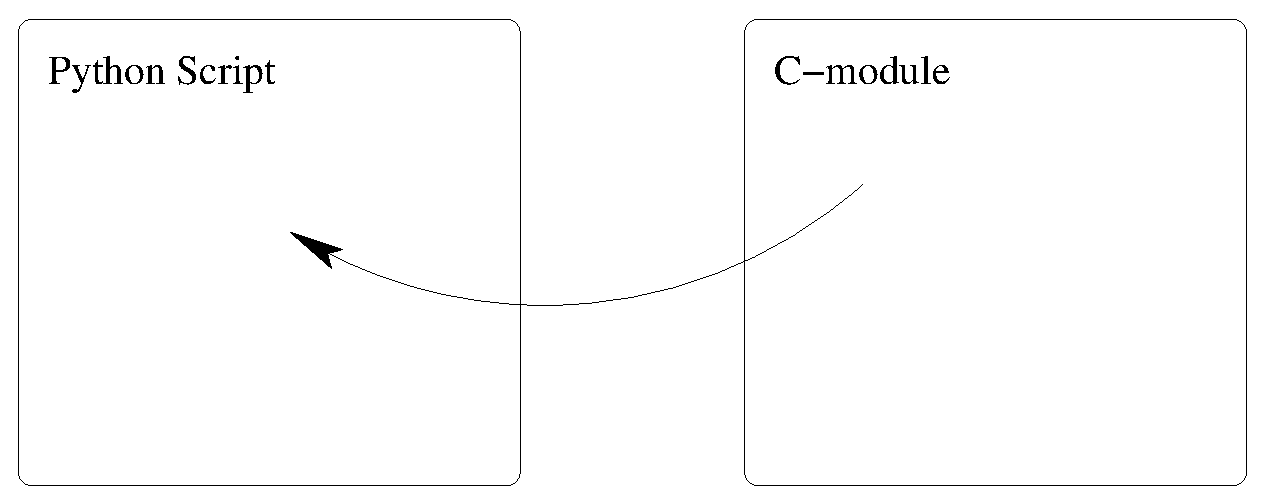
\includegraphics[width=.5\textwidth]{pics/cmod}

Python is implemented in C
\begin{itemize}
\item[\ra] all Python-datatypes are really C-structs
\end{itemize}

It is therefore necessary to
\begin{enumerate}
\item convert the arguments from the calling python-function to
  c-pointers (wrapper)
\item run the c-code
\item convert the result from the calculation to python-object and
  return to Python
\end{enumerate}

\end{frame}

%----------------------------------------------------------------------
%SLIDE -
\begin{frame}[fragile]{Roadmap for this talk}

\begin{block}{Roadmap}
  \begin{enumerate}
  \item Manual programming of wrapper-code
    \begin{itemize}
    \item directly accessing the python c-API
    \item includes compilation and linking of C-code
    \end{itemize}
  \item Automating this procedure
    \begin{itemize}
    \item using a wrapper-generator software (SWIG)
    \end{itemize}
  \item Alternatives for speedup
    \begin{itemize}
    \item {\tt scipy.weave}
    \item Cython
    \end{itemize}
  \end{enumerate}
\end{block}

\end{frame}


%----------------------------------------------------------------------
%SLIDE -
\section{Python C-API}

\begin{frame}[fragile]{Python's C-API}
  \framesubtitle{Python is C}

Python is implemented in C \ra you can access python's library from C
\begin{itemize}
\item allows to (1) embed python in your c-code and (2) to call c from python!
\item the python header must be included {\bf before} any other standard header!
  \begin{lstlisting}[language=c]
    #include "Python.h" 
  \end{lstlisting}
  \ra need to pass {\tt -I/path/to/python/include} to compiler

  \item all python-specific variables/functions start with the prefix
    {\tt Py}
  \item everything is a {\tt PyObject*}
  \item all Python objects have a type and a reference count
    \ra when an object's reference count becomes zero, the object is deallocated
\end{itemize}
\vfill
{\bf Everything else and more: \url{http://docs.python.org/c-api/}}
\end{frame}
%----------------------------------------------------------------------
%SLIDE -
\begin{frame}[fragile]{Python's C-API}
  \framesubtitle{different layers of abstraction}
  \begin{itemize}
    \item High-level, e.g. execute python code
      \begin{lstlisting}[language=c]
int PyRun_SimpleString(const char *command);
      \end{lstlisting}
    \item Abstract Object Layer, e.g. python's {\tt str(anything)}
      \begin{lstlisting}[language=c]
PyObject* PyObject_Str(PyObject *o);
      \end{lstlisting}
   \item Concrete Object Layer, e.g. conversion to python string
      \begin{lstlisting}[language=c]
PyObject* PyString_FromString(const char *v);
      \end{lstlisting}
  \end{itemize}
\vfill
{\bf Everything else and more: \url{http://docs.python.org/c-api/}}
\end{frame}
%----------------------------------------------------------------------
%SLIDE -


%----------------------------------------------------------------------
%SLIDE -
\section{Manually writing wrapper-code}

\begin{frame}{Writing a C-Extension}
Writing a python-module in c requires accessing the Abstract and
Concrete Object Layers.

  \begin{block}{Steps}
    \begin{enumerate}
    \item write and debug the C-function in terms of C-objects 
    \item write wrapper-code that specifies the python-interface to
      your code
    \item compile all C-sources into a shared object
    \item import and run the extension from Python
    \end{enumerate}
  \end{block}
  
\end{frame}


%----------------------------------------------------------------------
%SLIDE -
\begin{frame}[fragile]{Example 2: Primality-test}
  \framesubtitle{write and debug the C-function in terms of C-objects}

  Same as before

  \begin{lstlisting}[language=C,caption=prime.c]
int isprime( long num ){
  long i=2;
  while( i<num )
    if( num%i++==0 ) return 0;
  return 1;
}
  \end{lstlisting}

\end{frame}
%----------------------------------------------------------------------
%SLIDE -
\begin{frame}[fragile]{Example 2: Primality-test}
  \framesubtitle{write the wrapper code}

  \begin{lstlisting}[language=C,caption=primewrap.c]
#include <Python.h>

PyObject *wrap_isprime(PyObject *self, PyObject *args) {
  long num;
  if (!PyArg_ParseTuple(args,"l",&num))
      return NULL;
  return isprime(num) ? Py_True : Py_False;
}
  \end{lstlisting}

  
\end{frame}


%----------------------------------------------------------------------
%SLIDE -
\begin{frame}[fragile]{Example 2: Primality-test}
  \framesubtitle{register the module}

  \begin{lstlisting}[language=C,caption=primewrap.c continued]
...

static PyMethodDef primeMethods[] = {
  { "isprime", wrap_isprime, 1 },
  { NULL, NULL }
};


void initprimetest() {
  PyObject *m;
  m = Py_InitModule("primetest", primeMethods);
}
  \end{lstlisting}

  
\end{frame}
%----------------------------------------------------------------------
%SLIDE -
\begin{frame}[fragile]{Example 2: Primality-test}
  \framesubtitle{compile the module}

Likely to be different on your machine
  \begin{lstlisting}[language=bash,basicstyle=\footnotesize,caption=compilation]
$ gcc -fpic -c -I/usr/include/python2.7 primewrap.c\
          -o primetest.o
$ gcc -shared primetest.o -o primetestmodule.so
  \end{lstlisting}
\end{frame}
%----------------------------------------------------------------------
%SLIDE -
\begin{frame}[fragile]{Example 2: Primality-test}
  \framesubtitle{import and run the module from Python}

  \begin{lstlisting}[language=Python,basicstyle=\footnotesize,caption=test.py]
from primetest import isprime
print isprime(715827883)
  \end{lstlisting}

\ra Runtime: 7.488 sec
\end{frame}
%----------------------------------------------------------------------
%SLIDE -

\section{SWIG}

\begin{frame}{SWIG - Simplified Wrapper and Interface
    Generator}

\begin{itemize}
\item A compiler that turns ANSI C/C++ declarations into scripting language interfaces.
\item Completely automated (produces a fully working Python extension module).
\item Language neutral. SWIG can also target Tcl, Perl, Guile, MATLAB, etc...
\item Attempts to eliminate the tedium of writing extension modules.
\end{itemize}

\centering
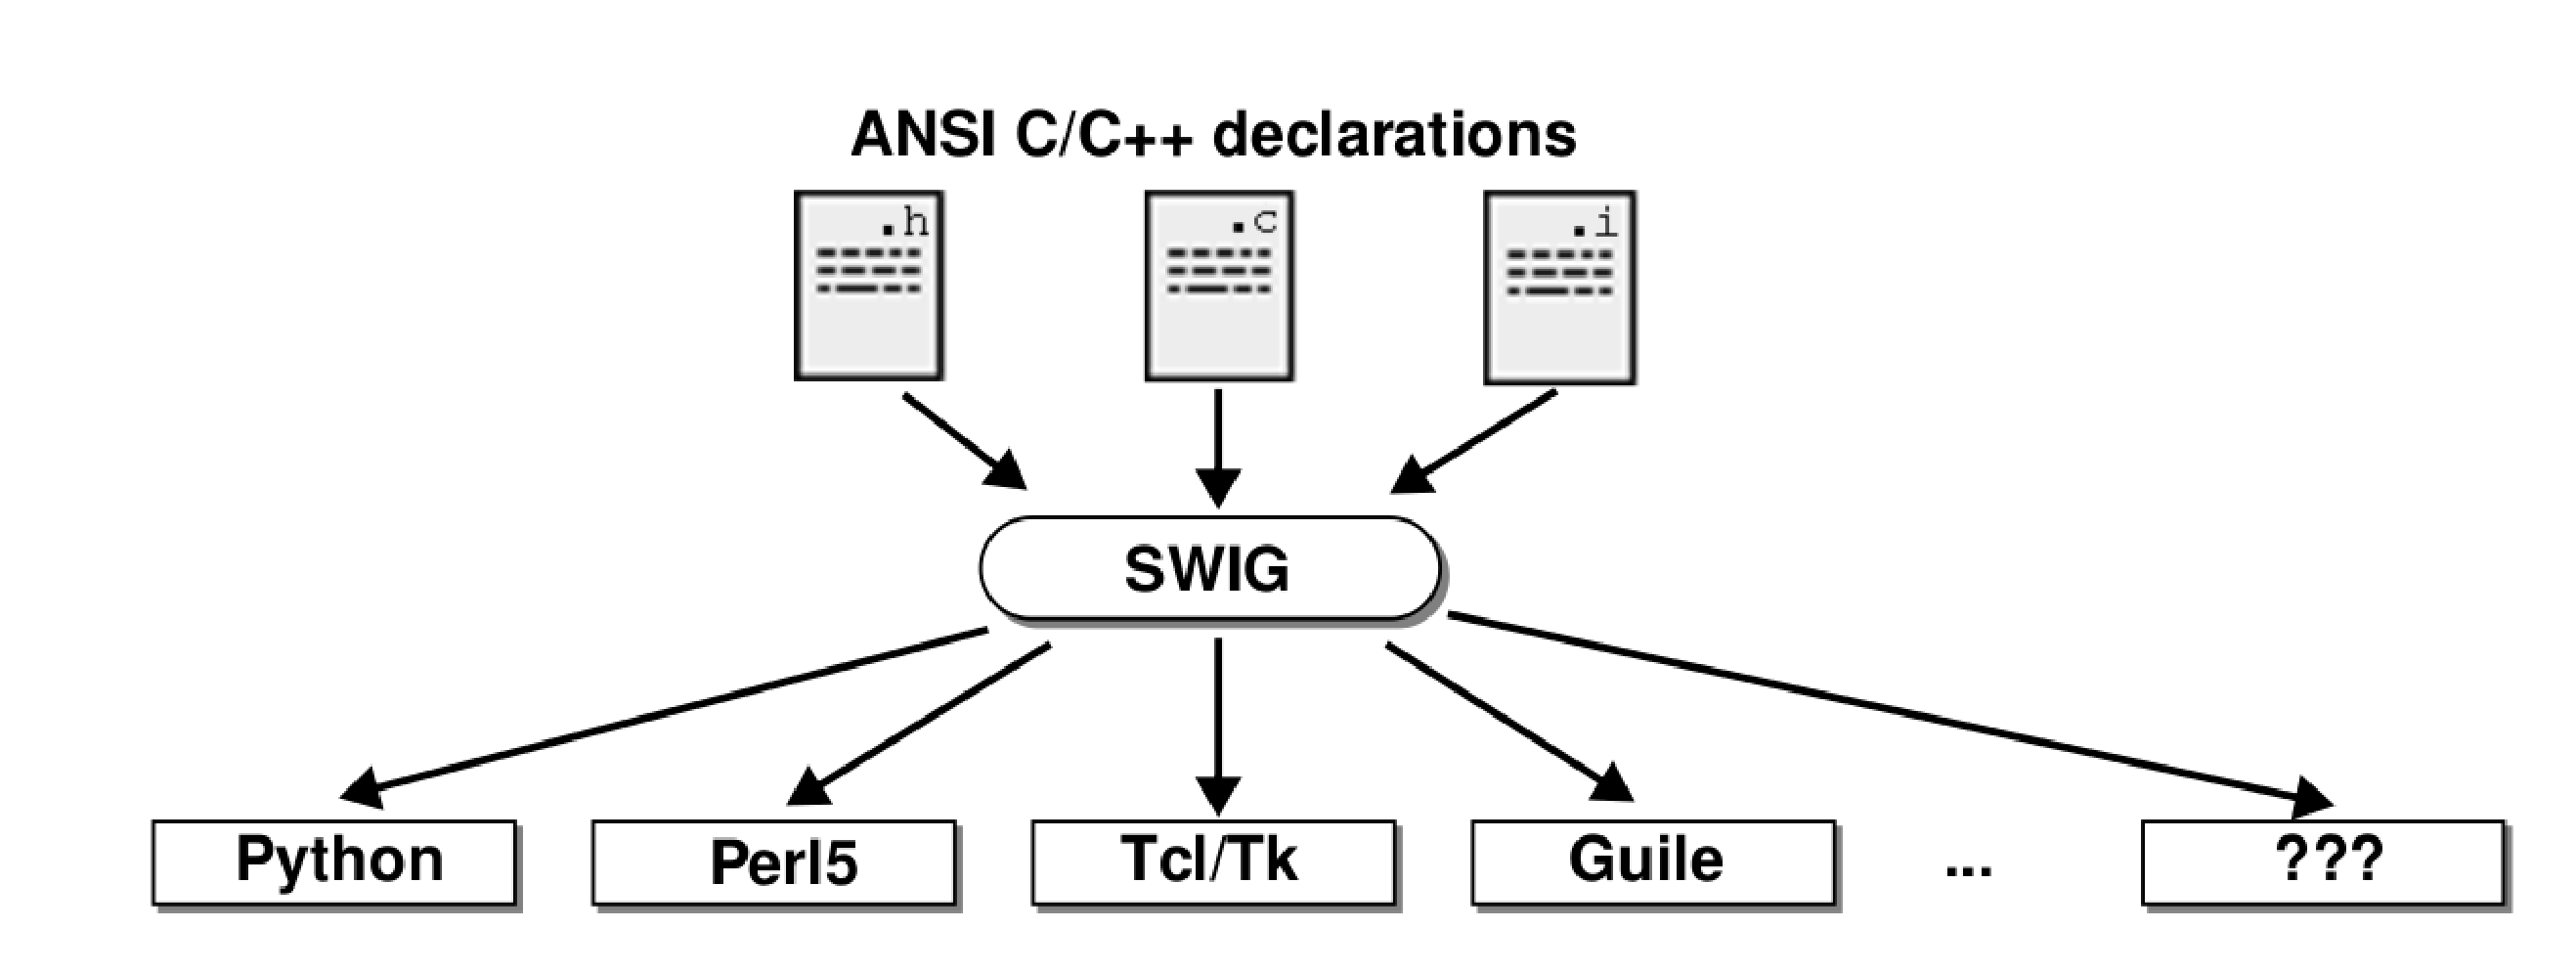
\includegraphics[width=\textwidth]{pics/swigstructure}
\end{frame}
%----------------------------------------------------------------------
%SLIDE -
\begin{frame}[fragile]{SWIG'ified Primality test}

  We need a special interface-file (.i) that specifies the interface
  to generate:
%  \lstinputlisting[language=C,caption=primetest.c]{../primetest.c}
  \lstinputlisting[language=C,caption=primetest.i]{../examples/prime/primetest.i}

\vfill
  Now we just need to run SWIG and compile the example:
  \begin{lstlisting}[language=bash]
$ swig -python primetest.i 
$ gcc -fPIC -c primetest.c primetest_wrap.c\ 
                   -I/usr/include/python2.7
$ gcc -shared primetest.o primetest_wrap.o\
                   -o _primetest.so
  \end{lstlisting}
\end{frame}
%----------------------------------------------------------------------
%SLIDE -

\begin{frame}{SWIG'ified Primality test}
  Result:
  \begin{itemize}
  \item the wrapper code is completely generated by SWIG
  \item in this example, only the c-function specification had to be
    given
  \item still, we had to compile the code manually
  \item[\ra] enter python {\tt distutils}\ldots
  \end{itemize}
\end{frame}
%----------------------------------------------------------------------
%SLIDE -

\begin{frame}[fragile]{Python distutils}
  \framesubtitle{Python's Makefiles}
  Python package {\tt distutils} provides functionality similar to
  {\tt Makefiles}.

  \begin{itemize}
  \item write a python file {\tt setup.py}
  \item specify the dependencies in this file
  \item run {\tt python setup.py install} to install the module
  \end{itemize}

  \begin{lstlisting}[language=bash,basicstyle=\tiny]
$ python setup.py --help-commands
Standard commands:
  build            build everything needed to install
  build_py         "build" pure Python modules (copy to build directory)
  build_ext        build C/C++ extensions (compile/link to build directory)
  build_clib       build C/C++ libraries used by Python extensions
  build_scripts    "build" scripts (copy and fixup #! line)
  clean            clean up temporary files from 'build' command
  install          install everything from build directory
  install_lib      install all Python modules (extensions and pure Python)
  install_headers  install C/C++ header files
  install_scripts  install scripts (Python or otherwise)
  install_data     install data files
  sdist            create a source distribution (tarball, zip file, etc.)
  register         register the distribution with the Python package index
  bdist            create a built (binary) distribution
  bdist_dumb       create a "dumb" built distribution
  bdist_rpm        create an RPM distribution
  bdist_wininst    create an executable installer for MS Windows
  upload           upload binary package to PyPI
  check            perform some checks on the package
  \end{lstlisting}
  
\end{frame}
%----------------------------------------------------------------------
%SLIDE -

\begin{frame}[fragile]{setup.py}

{\bf Step 1:} write setup.py
\lstinputlisting[caption=prime/setup.py]{../examples/prime/setup.py}
{\bf Step 2:} build module and test import
\begin{lstlisting}[language=bash,basicstyle=\tiny]
$ python setup.py build_ext -i
running build_ext
building '_primetest' extension
swigging primetest.i to primetest_wrap.c
swig -python -o primetest_wrap.c primetest.i
creating build
creating build/temp.linux-x86_64-2.7
gcc -pthread -fno-strict-aliasing [...] (truncated)
gcc -pthread -shared -Wl, [...] (truncated)
$ python -c "import primetest"
\end{lstlisting}

\end{frame}
%----------------------------------------------------------------------
%SLIDE -

\begin{frame}{SWIG output}

{\centering
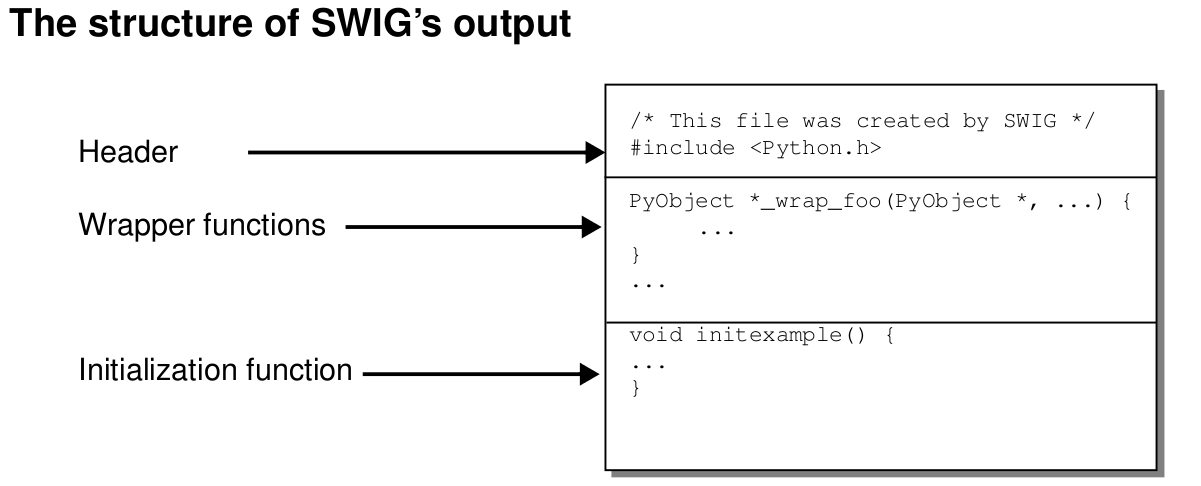
\includegraphics[width=.9\textwidth]{pics/swigoutput}}

Four directives are available for inserting code
\begin{itemize}
\item {\tt \%\{ ... \%\}} inserts code into the header section.
\item {\tt \%wrapper \%\{ \ldots \%\}} inserts code into the wrapper section.
\item {\tt \%init \%\{ \ldots \%\}} inserts code into the initialization function.
\item {\tt \%inline \%\{ \ldots \%\}} inserts code into the header
%  section and 
  %wraps it.
\end{itemize}
\end{frame}
%----------------------------------------------------------------------
%SLIDE -

\begin{frame}{SWIG}

{\bf Datatypes}: C built-in datatypes are mapped into the closest
Python equivalent.

\begin{itemize}
\item int, long, short $\Leftrightarrow$ Python integers.
\item float, double $\Leftrightarrow$ Python floats
\item char, char * $\Leftrightarrow$ Python strings.
\item void $\Leftrightarrow$ None
\item long long, long double \ra Currently unsupported
\end{itemize}

\end{frame}
%----------------------------------------------------------------------
%SLIDE -


\begin{frame}[fragile]{Pointers}
As long as we do not need to know anything about the pointers, we can
just pass them between functions\ldots

\begin{lstlisting}[language=C,caption=example.i]
%module example
FILE* fopen(char *filename, char *mode);
int fclose(FILE *f);
\end{lstlisting}
translates to
\begin{lstlisting}[language=python,caption=testexample.py]
import example
f=example.fopen( "test.csv", "r")
example.fclose(f)
\end{lstlisting}
\end{frame}
%----------------------------------------------------------------------
%SLIDE -

\begin{frame}[fragile]{SWIG}
You guessed it: 

\begin{center}
  {\bf Problem: What about complex datatypes, e.g. list, dictionaries,
    numpy-arrays etc?}
\end{center}
There is no easy way to pass arbitrary lists, e.g.

\begin{lstlisting}
[ (1,2,3), {'a':"this is a string"}, ['a', 'b', 2] ]
\end{lstlisting}
to C.

Fortunately, for scientific application, we will usually want to pass
numpy-arrays. This is relatively simple, because they are
arrays of identical objects and can easily be translated to pointers.

\begin{itemize}
\item {\tt np.array([1,2,3], dtype=np.float32)} $\Leftrightarrow$ {\tt
  (float*)malloc(3*sizeof(float))}
\item \ldots
\end{itemize}

\end{frame}

%----------------------------------------------------------------------
%SLIDE -
\begin{frame}[fragile]{SWIG and numpy}
Say we have a c-function for calculating a vector norm
\lstinputlisting[language=c,caption=vnorm.c]{../examples/vnorm/vnorm.c}
A convenient interface from python would be using numpy-arrays
\begin{lstlisting}
import numpy, vnorm
n=vnorm.vnorm( numpy.random.rand(100) )
\end{lstlisting}
\ldots which requires that the data-pointer is mapped to {\tt *vec} and
the length of the input array is mapped to {\tt lvec} in the c-wrapper

Fortunately, there is a mechanism for that\ldots

\end{frame}
%----------------------------------------------------------------------
%SLIDE -


\begin{frame}[fragile]{SWIG: numpy.i}
Interface file {\tt numpy.i}, documentation at 
\url{http://docs.scipy.org/doc/numpy/reference/swig.interface-file.html}

Provides many SWIG-{\tt typemaps} to transform numpy arrays to
c-pointers, e.g.
\begin{lstlisting}[language=c]
%apply (double* IN_ARRAY1, int DIM1) {(double* vec, int lvec)};
\end{lstlisting}
Basically, this generates code in the wrapper of the form 
\begin{lstlisting}[language=c]
  ...
    arg1 = (double*) array_data(array1);
    arg2 = (int) array_size(array1,0);
    result = (double)vnorm(arg1,arg2);
  ...
\end{lstlisting}
i.e. extracting and assigning pointers and size of the arrays to the
proper variables.
\end{frame}

%----------------------------------------------------------------------
%SLIDE -
\begin{frame}[fragile]{SWIG: numpy.i}
\framesubtitle{vector norm implementation}
\lstinputlisting[language=c,caption=vnorm.i]{../examples/vnorm/vnorm.i}
\end{frame}
%----------------------------------------------------------------------
%SLIDE -
\begin{frame}[fragile]{SWIG: numpy.i}
\framesubtitle{using vector norm package}

Using the module is now fairly easy
\lstinputlisting[language=c,caption=testvnorm.py,basicstyle=\tiny]{../examples/vnorm/testvnorm.py}
\begin{lstlisting}[language=bash,caption=output]
18.607797232 18.607797232 18.607797232
7.14142842854 7.14142842854 7.14142842854
1005.03781023 1005.03781023 1005.03781023
\end{lstlisting}
and it even works for all iterable objects (thanks to SWIG)!
\end{frame}

%----------------------------------------------------------------------
%SLIDE -

\begin{frame}{Example 3: Dynamic Time Warping (DTW)}
  \framesubtitle{What is the shortest path through a matrix?}
 
  \begin{minipage}{.43\textwidth}
    \hspace{-1.5cm}
    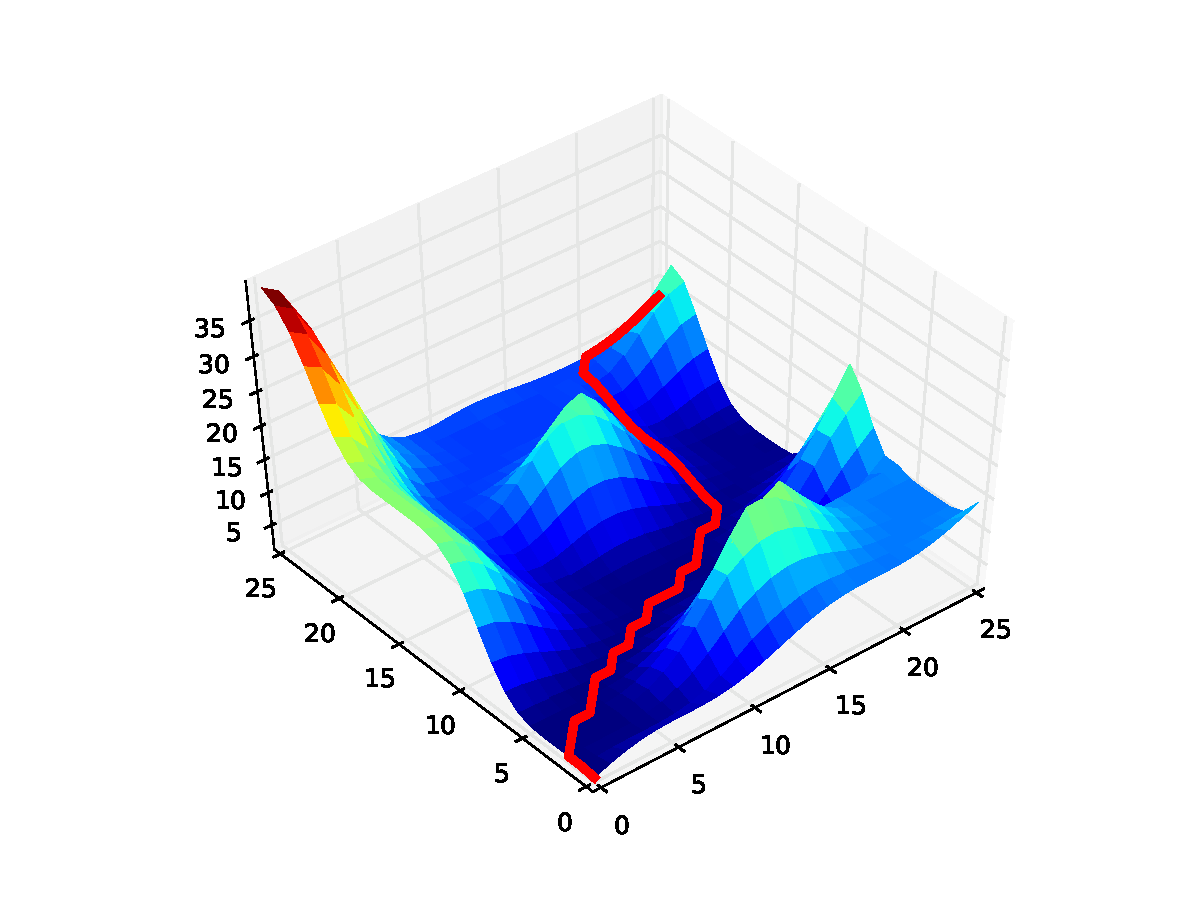
\includegraphics[width=1.5\textwidth]{pics/dtwexample}
  \end{minipage}
  \hfill
  \begin{minipage}{.55\textwidth}
    \begin{block}{Algorithm 2: DTW}
      Given a $N_1 \times N_2$ matrix $\mathbf{M}$, the (gapless) path $\mathbf{p}=(\vec{p},\vec{q})$
      from $(0,0)$ to $(N_1,N_2)$ minimizing $\sum_{i,j\in
        \mathbf{p}}{\mathbf{M}_{i,j}}$ can be found as follows
      \begin{itemize}
      \item calculate
        $\mathbf{D}_{i,j}=\mathbf{M}_{i,j}+\min{\left\{\mathbf{D}_{i,j-1},\mathbf{D}_{i-1,j},\mathbf{D}_{i-1,j-1}\right\}}$
      \item Given $(p_1, q_1)=(N_1,N_2)$, $(p_{i+1},q_{i+1}) = (j,k)$
        s.t.$ \mathbf{D}_{j,k}=\min\left\{ \mathbf{D}_{p_i,q_i-1},
        \mathbf{D}_{p_i-1,q_i},  \mathbf{D}_{p_i-1,q_i-1} \right\}$
      \end{itemize}
    \end{block}
  \end{minipage}
  \begin{block}{Properties of this example}
    \begin{itemize}
    \item computationally intense, requires passing
      matrices back and forth
    \item cannot efficiently done in numpy because of recursion
    \end{itemize}
  \end{block}
\end{frame}

%------------------------------------------------------mmmmmmmmmmm----------------
%SLIDE -
\begin{frame}[fragile]{Example 3: DTW}
\framesubtitle{Pure Python}
\begin{lstlisting}[language=Python,basicstyle=\tiny]
def dtw( M ):
    """Given a matrix M, calculate the shortest path between (0,0) and (N1,N2)"""
    N1,N2=M.shape
    D=M.copy()
    for i in range(N1-1):
        for j in range(N2-1):
            D[i+1,j+1]=M[i,j]+min([D[i,j+1],D[i+1,j],D[i+1,j+1]])

    p1,p2=([N1-1],[N2-1])
    while p1[0]>0 or p2[0]>0:
        i,j=(p1[0],p2[0]) 
        midx=np.argmin( np.array( \
            [ D[i-1,j  ] if i>0 else np.inf, \
              D[i,j-1  ] if j>0 else np.inf, \
              D[i-1,j-1] if i>0 and j>0 else np.inf]))
        if midx==0:
            p1.insert(0,i-1)
            p2.insert(0,j  )
        elif midx==1:
            p1.insert(0,i  )
            p2.insert(0,j-1)
        else:
            p1.insert(0,i-1)
            p2.insert(0,j-1)
            
    return D,np.array([p1,p2])
\end{lstlisting}
\end{frame}
%----------------------------------------------------------------------
%SLIDE -

\begin{frame}[fragile]{SWIG: numpy.i}
\framesubtitle{DTW example}
Say, we have a C-implementation of DTW
\begin{lstlisting}[language=c,caption=cdtw.c]
int cdtw( double *M, int n1, int n2, 
          int *p, int nd, int np ){
  ...
  return 0;
}
\end{lstlisting}
where the input matrix is M of dimension n1 $\times$ n2 and p is the
output path.

Define a typemap that maps this to python:
\begin{lstlisting}[language=c,basicstyle=\tiny,caption=cdtw.i]
...
%apply (double* IN_ARRAY2, int DIM1, int DIM2) 
    {(double* M, int n1, int n2)};
%apply (int* INPLACE_ARRAY2, int DIM1, int DIM2) 
    {(int* p, int nd, int np)};
int cdtw( double *M, int n1, int n2, 
          int *p, int nd, int np );
...
\end{lstlisting}
\end{frame}
%----------------------------------------------------------------------
%SLIDE -
\begin{frame}[fragile]{SWIG: numpy.i}
\framesubtitle{DTW example cont'd}
We can now call cdtw from python, BUT we have to allocate the output
ourselves, e.g.
\begin{lstlisting}[language=Python]
from cdtw import *
M=some_matrix()
n1,n2=M.shape
p=np.ones( (2,n1+n2), dtype=np.int32)
cdtw( M, p )
# p is now the output path (in-place)
\end{lstlisting}

Nice SWIG-feature: We can put such code into the interface file\ldots
\end{frame}
%----------------------------------------------------------------------
%SLIDE -
\begin{frame}[fragile]{SWIG: numpy.i}
\framesubtitle{DTW example cont'd}
\begin{lstlisting}[language=c,caption=cdtw.i cont'd,basicstyle=\tiny]
...
/* Rewrite the high level interface to cdtw */
%pythoncode %{
import numpy as np
def cdtw(M):
  n1,n2=M.shape
  p=-1*np.ones( (2,2*n1), dtype=np.int32)
  _cdtw.cdtw(M, p)
  p=np.row_stack( (p[0,:][(p[0,:]>=0)][::-1], p[1,:][(p[1,:]>=0)][::-1]))
					
  return p
%}
\end{lstlisting}
This code overwrites the previous {\tt cdtw()} declaration, so that we
have the desired interface, i.e.
\begin{lstlisting}[language=python]
from cdtw import *
M=some_matrix()
p=cdtw( M )
\end{lstlisting}
\end{frame}
%----------------------------------------------------------------------
%SLIDE -
\begin{frame}[fragile]{DTW runtime comparison}
  Running python vs. c implementation for matrices of varying size
  (see {\tt dtw\_runtime.py})
{  \centering
  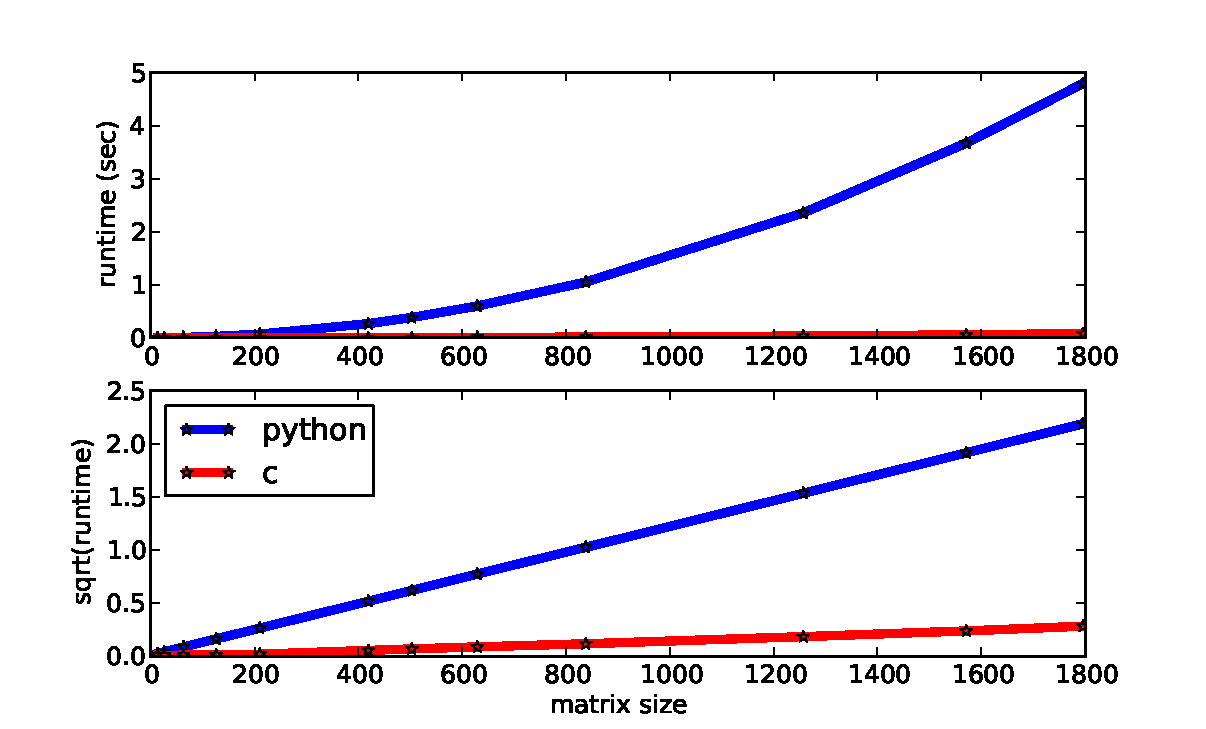
\includegraphics[width=.8\textwidth]{pics/dtw_cvspython}}

\ra python implementation is quickly getting unusable
\end{frame}
%----------------------------------------------------------------------
%SLIDE -

\section{weave.inline}
\begin{frame}[fragile]{weave.inline}
  \begin{lstlisting}[language=Python,basicstyle=\footnotesize]
import scipy.weave as w
a=13
w.inline('printf("This is printf from C, a=%i", a);', ['a'])
  \end{lstlisting}
  \begin{itemize}
  \item directly execute c-code from within python
  \item code is compiled the first time you run the script
  \end{itemize}
\end{frame}
%----------------------------------------------------------------------
%SLIDE -

\begin{frame}[fragile]{weave.inline}
  \framesubtitle{Primality test once again}
  These things said, let's look at our example:
  \lstinputlisting[language=Python,basicstyle=\footnotesize,caption=prime\_weave.py]{../examples/prime/prime_weave.py}
  
{\bf  Timing: 6.957 sec}
\end{frame}
%----------------------------------------------------------------------
%SLIDE -
\begin{frame}[fragile]{weave.inline}
  \framesubtitle{Issues\ldots}
  Seems to be easy, but really is not:
  \begin{itemize}
  \item for more complex data (lists, numpy-arrays, \ldots), you need
    to know the C-API
  \item uses PyCXX datatypes (a separate library that wraps python
    datatype to C++) $\ra$ another syntax to learn
  \item you need to keep track of references/garbage yourself
  \item different versions work or work not with the same code
    (believe me, I've been there) \ra my examples use the most recent
    versions of numpy/scipy (upgrade your system as follows)
    \begin{lstlisting}[language=bash]
$ easy_install -U numpy
$ easy_install -U scipy
    \end{lstlisting}
  \item the current documentation at
    \url{http://docs.scipy.org/doc/scipy-0.10.1/reference/tutorial/weave.html}
    is incorrect, you need to figure it out yourself
  \end{itemize}
\end{frame}
%----------------------------------------------------------------------
%SLIDE -
\begin{frame}[fragile]{weave.inline}
  \framesubtitle{Variable conversion}
{\tt py::} types are from the PyCXX-library

\begin{tabular}{l|l}
Python &	C++\\\hline
int &	int\\
float	 &double\\
complex &	std::complex\\
string &	py::string\\
list &	py::list\\
dict &	py::dict\\
tuple &	py::tuple\\
file &	FILE*\\
callable &	py::object\\
instance &	py::object\\
numpy.ndarray &	PyArrayObject*\\
\end{tabular}
\end{frame}
%----------------------------------------------------------------------
%SLIDE -

\begin{frame}[fragile]{weave.inline}
  \framesubtitle{}
  \begin{itemize}
  \item there is no return, instead return values are assigned to a
    special variable {\tt return\_val}
  \item this variable is of type {\tt py::object} (basic types are
    automatically converted)
  \item no function definitions (the code is wrapped into a function
    as a whole and C does not allow functions in functions)
  \end{itemize}

  \begin{block}{Conclusion}
    Fast to write (just one file) and maybe good for quick
    jobs.

    Can become really tedious, though\ldots
  \end{block}
\end{frame}
%----------------------------------------------------------------------
%SLIDE -

\section{Cython}
\begin{frame}[fragile]{Cython}
  \framesubtitle{Optimize from within python}
  
\includegraphics[width=.3\textwidth]{pics/cython}
  \begin{block}{Idea: Cython is\ldots}
    \ldots a programming language based on Python, with extra syntax
    allowing for optional static type
    declarations
  \end{block}
  \begin{itemize}
  \item uses source code compiler that translates Python code to
    equivalent C code
  \item c-code is executed within the python runtime environment, but
    at the speed of compiled C and with the ability to call directly
    into C libraries.
  \end{itemize}
\end{frame}
%----------------------------------------------------------------------
%SLIDE -

\begin{frame}[fragile]{Cython}
  \framesubtitle{Very short overview}
  \begin{itemize}
  \item cython files end with {\tt .pyx}
  \item compilation still necessary:
\begin{lstlisting}[caption=setup.py,basicstyle=\tiny]
from distutils.core import setup
from distutils.extension import Extension
from Cython.Distutils import build_ext

setup(
    cmdclass = {'build_ext': build_ext},
    ext_modules = [Extension("helloworld", ["helloworld.pyx"])]
)
\end{lstlisting}
\item special keywords for defining c-variables
\begin{lstlisting}
cdef int i,j,k
cdef float *data
cdef int myfunction( int x, float y ):
cdef class TigerEatingLion:
\end{lstlisting}
  \end{itemize}
\end{frame}
%----------------------------------------------------------------------
%SLIDE -

\begin{frame}[fragile]{Cython}
  \framesubtitle{Very short overview}
  \begin{itemize}
  \item can result in dramatic speedups (similar to pure c-extension
    modules)
  \item you need to be clear about the compilation process in order to
    exploit cython's capabilities:
    \begin{lstlisting}
cdef int i,k,n
cdef int p[1000]
...
while i < k and n % p[i] != 0:
   i = i + 1
    \end{lstlisting}
    is very fast even though it is a python while-loop because it does
    not contain python-types
  \item[\ra] care must be taken to avoid mixing cdef and python types!
  \end{itemize}
\end{frame}
%----------------------------------------------------------------------
%SLIDE -

\setbeamercovered{transparent=20}
%% Table of Contents
\begin{frame}{Link Collection}

\begin{itemize}
\item \url{http://docs.python.org/c-api/}
\item \url{http://docs.scipy.org/doc/numpy/reference/c-api.html}
\item \url{http://docs.scipy.org/doc/numpy/reference/swig.interface-file.html}
\item \url{http://www.scipy.org/Weave}
\item \url{http://starship.python.net/crew/theller/ctypes/} for
  passing c-types to c-functions from python
\item \url{http://cython.org/}

\end{itemize}

\end{frame}
\setbeamercovered{invisible}

\end{document}

